% Created 2016-08-17 Wed 14:38
\documentclass[tikz]{standalone}

\usepackage[utf8]{inputenc}
\usepackage[T1]{fontenc}
\usepackage{marvosym}

\usepackage{helvet}
\usepackage{../../templates/msc}
\usepackage{tikzsymbols}
\usepackage{tikzpeople}
\usepackage{comment}

\renewcommand{\familydefault}{\sfdefault}


\usetikzlibrary{intersections}
\usepackage{xparse}


\usepackage{../../templates/networkSymbols}

\tikzset{
  every picture/.style={
    line width=1pt
  },
  % database/.style={
  %   cylinder,
  %   cylinder uses custom fill,
  %   cylinder body fill=yellow!50,
  %   cylinder end fill=yellow!50,
  %   shape border rotate=90,
  %   aspect=0.25,
  %   draw
  % },
  % from: https://tex.stackexchange.com/questions/41533/is-there-a-tikz-library-for-network-symbols 
  % interface/.style={draw, rectangle, rounded corners, font=\LARGE\sffamily}    ,
  % ethernet/.style={interface, fill=yellow!50},% ethernet interface
  % serial/.style={interface, fill=green!70},% serial interface
  % speed/.style={sloped, anchor=south, font=\large\sffamily},% line speed at edge
  % route/.style={draw, shape=single arrow, single arrow head extend=4mm,
  %   minimum height=1.7cm, minimum width=3mm, white, fill=blue!20,
  %   drop shadow={opacity=.8, fill=blue!50!black}, font=\tiny}% inroute / outroute arrows
}




\author{Holger Karl}
\date{\today}
\title{}




\begin{document}

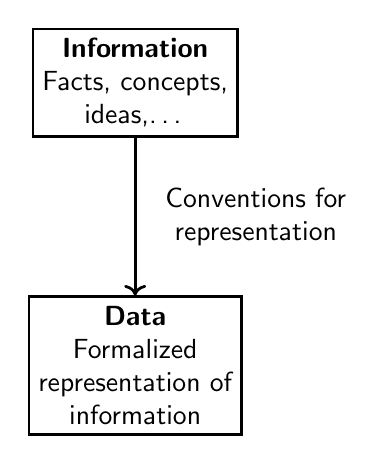
\begin{tikzpicture}
  \node[align=center, draw] (inf)  {\textbf{Information}\\ Facts, concepts,\\ideas,\dots}; 
  \node[align=center, draw, below=2cm of inf] (data)  {\textbf{Data}\\  Formalized \\representation of\\information}; 

  \draw [->] (inf) to node[align=center, midway, right=0.25cm] {Conventions for\\ representation} (data); 
\end{tikzpicture}

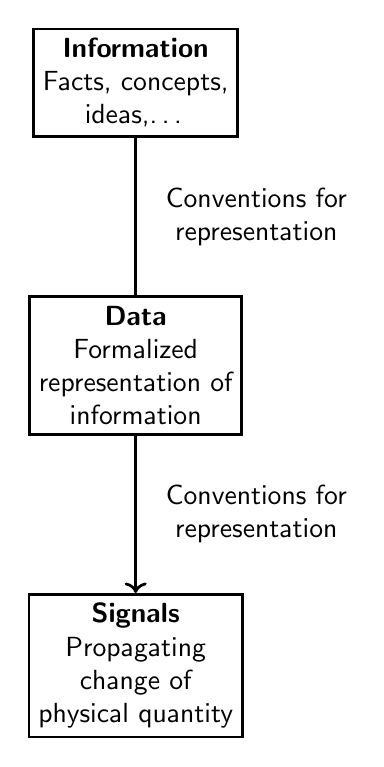
\begin{tikzpicture}
  \node[align=center, draw] (inf)  {\textbf{Information}\\ Facts, concepts,\\ideas,\dots}; 
  \node[align=center, draw, below=2cm of inf] (data)  {\textbf{Data}\\  Formalized \\representation of\\information}; 
  \node[align=center, draw, below=2cm of data] (signal)  {\textbf{Signals}\\  Propagating\\ change of \\physical quantity}; 

  \draw [->] (inf) to node[align=center, midway, right=0.25cm]
  {Conventions for\\ representation}
  (data)to node[align=center, midway, right=0.25cm]
  {Conventions for\\ representation} (signal); 
\end{tikzpicture}




\end{document}